% Source: AESP_466_ClassWork/Exams/Midterm/AESP466_Midterm_Sp26_rev1b.tex

\documentclass[border=4pt]{standalone}
\usepackage{amsmath}
\usepackage{amssymb}
\usepackage{graphicx}
\usepackage{tikz}
\usepackage{xcolor}

\definecolor{Garnet}{HTML}{73000A}
\definecolor{USC_Rose}{HTML}{CC2E40}
\definecolor{USC_Blue}{HTML}{466A9F}
\definecolor{USC_Slate}{HTML}{1F414D}
\definecolor{USC_Olive}{HTML}{65780B}
\definecolor{USC_Black90}{HTML}{565656}
\definecolor{USC_Black10}{HTML}{ECECEC}

\begin{document}
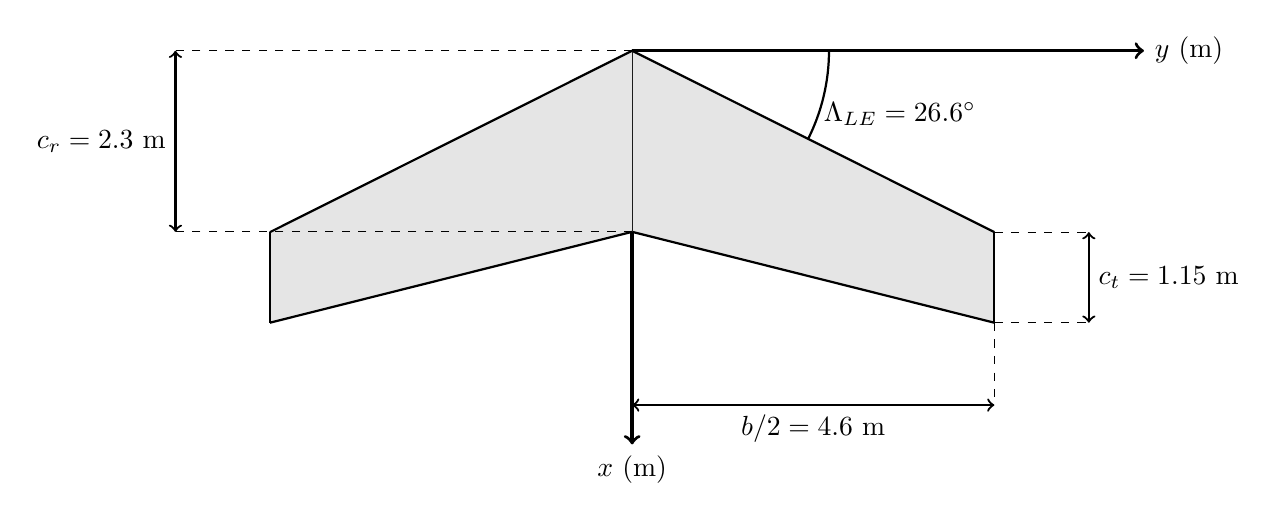
\begin{tikzpicture}[scale=1.0]
% Coordinate system at wing apex (LE of root)
\draw[->, very thick] (0,0) -- (0,-5) node[below] {$x$ (m)};
\draw[->, very thick] (0,0) -- (6.5,0) node[right] {$y$ (m)};
% Right half-wing
\fill[gray!20] (0,0) -- (4.6,-2.304) -- (4.6,-3.454) -- (0,-2.3) -- cycle;
\draw[thick] (0,0) -- (4.6,-2.304);          % Leading edge
\draw[thick] (0,-2.3) -- (4.6,-3.454);       % Trailing edge
\draw[thick] (0,0) -- (0,-2.3);              % Root chord
\draw[thick] (4.6,-2.304) -- (4.6,-3.454);   % Tip chord
% Left half-wing (mirror)
\fill[gray!20] (0,0) -- (-4.6,-2.304) -- (-4.6,-3.454) -- (0,-2.3) -- cycle;
\draw[thick] (0,0) -- (-4.6,-2.304);
\draw[thick] (0,-2.3) -- (-4.6,-3.454);
\draw[thick] (-4.6,-2.304) -- (-4.6,-3.454);
% Dimension: root chord
\draw[dashed, thin] (0,0) -- (-5.8,0);
\draw[dashed, thin] (0,-2.3) -- (-5.8,-2.3);
\draw[<->, thick] (-5.8,0) -- (-5.8,-2.3);
\node[left] at (-5.8,-1.15) {$c_r = 2.3$ m};
% Dimension: tip chord
\draw[dashed, thin] (4.6,-2.304) -- (5.8,-2.304);
\draw[dashed, thin] (4.6,-3.454) -- (5.8,-3.454);
\draw[<->, thick] (5.8,-2.304) -- (5.8,-3.454);
\node[right] at (5.8,-2.879) {$c_t = 1.15$ m};
% Dimension: semi-span
\draw[dashed, thin] (0,-3.454) -- (0,-4.5);
\draw[dashed, thin] (4.6,-3.454) -- (4.6,-4.5);
\draw[<->, thick] (0,-4.5) -- (4.6,-4.5);
\node[below] at (2.3,-4.5) {$b/2 = 4.6$ m};
% Sweep angle arc
\draw[dashed] (0,0) -- (3.5,0);
\draw[thick] (2.5,0) arc (0:-26.6:2.5);
\node at (3.4,-0.8) {$\Lambda_{LE} = 26.6^\circ$};
\end{tikzpicture}
\end{document}
